\subsection{Matrices del sistema}
La matriz $\Lambda$ de coeficientes de desintegración del sistema es un arreglo disperso. A continuación se muestra dejando en blanco aquellos elementos valuados en 0:

\begin{equation}
	\Lambda=\left(\begin{smallmatrix}
		-\lambda_1& & & & & & & & & & & & & & \\
		 \lambda_1&-\lambda_2& & & & & & & & & & & & & \\
		 & \lambda_2&-\lambda_3& & & & & & & & & & & & \\
		 & & \lambda_3&-\lambda_4& & & & & & & & & & & \\
		 & & &\lambda_{4,\beta}&-\lambda_5& & & & & & & & & & \\
		 & & &\lambda_{4, \alpha}& &-\lambda_6& & & & & & & & & \\
		 & & & & \lambda_5& \lambda_6&-\lambda_7& & & & & & & & \\
		 & & & & & & \lambda_7&-\lambda_8& & & & & & & \\
		 & & & & & & & \lambda_8&-\lambda_9& & & & & & \\
		 & & & & & & & &\lambda_{9,\alpha}&-\lambda_{10}& & & & & \\
		 & & & & & & & &\lambda_{9, \beta}& &-\lambda_{11}& & & & \\
		 & & & & & & & & & \lambda_{10}&\lambda_{11}&-\lambda_{12}& & & \\
		 & & & & & & & & & & &\lambda_{12, \beta}&-\lambda_{13}& & \\
		 & & & & & & & & & & &\lambda_{12, \alpha}& &-\lambda_{14}& \\ 
		 & & & & & & & & & & & &\lambda_{13}&\lambda_{14}& 0\\
	\end{smallmatrix}\right)
\end{equation}\label{matriz_determinista}

Para la versión estocástica del sistema, se toma como término determinista la matriz $\mathcal{L}$ y las matrices estocásticas $\mathcal{X}$, $\mathcal{Y}$ y $\mathcal{Z}$ dadas por los siguientes arreglos dispersos:

\begin{equation}
	\mathcal{L}=\left(\begin{smallmatrix}
		-\lambda_1& & & & & & & & & & & \\								%fila 1
		\lambda_1&-\lambda_2& & & & & & & & & & \\						%fila 2
		&\lambda_2&-\lambda_3& & & & & & & & & \\						%fila 3
		& & \lambda_3&-\lambda_4& & & & & & & & \\						%fila 4
		& & &\lambda_{4, \alpha}&-\lambda_6& & & & & & & \\				%fila 5
		& & & &\lambda_6 &-\lambda_7& & & & & & \\						%fila 6
		& & & & &\lambda_7&-\lambda_8& & & & & \\						%fila 7
		& & & & & &\lambda_8&-\lambda_9& & & & \\						%fila 8
		& & & & & & &\lambda_{9, \beta}&-\lambda_{11}& & & \\			%fila 9
		& & & & & & & &\lambda{11}&-\lambda_{12}& & \\					%fila 10
		& & & & & & & & &\lambda_{12, \beta}&-\lambda_{14}&\\			%fila 11 
		& & & & & & & & & &\lambda{14}& 0\\								%fila 12
	\end{smallmatrix}\right)
\end{equation}\label{matriz_determinista_alternativa}

\begin{equation}
	\mathcal{X}=\begin{cases}
		(\lambda_4-2\lambda_{4, \alpha}) & \textrm{En la fila 5, columna 4.}\\
		-\lambda_5+\lambda_6 & \textrm{En la fila 5, columna 5.}\\
		\lambda_5-\lambda_6 & \textrm{En la fila 6, columna 5.}
	\end{cases}
\end{equation}\label{matriz_estocastica_x}

\begin{equation}
	\mathcal{Y}=\begin{cases}
		-(\lambda_9-2\lambda_{9, \alpha}) & \textrm{En la fila 9, columna 8.}\\
		-\lambda_{10}+\lambda_{11} & \textrm{En la fila 9, columna 9.} \\
		\lambda_{10}-\lambda_{11} & \textrm{En la fila 10, columna 9.} \\
	\end{cases}
\end{equation}\label{matriz_estocastica_y}

\begin{equation}
	\mathcal{Z}=\begin{cases}
		(\lambda_{12}-2\lambda_{12, \alpha}) & \textrm{En la fila 11, columna 10.}\\
		-\lambda_{13}+\lambda_{14} & \textrm{En la fila 11, columna 11.}\\
		\lambda_{13}-\lambda_{14}  & \textrm{En la fila 12, columna 11.}\\
	\end{cases}
\end{equation}\label{matriz_estocastica_z}

\noindent donde se suponen 0 todos los elementos no especificados.

\subsection{Tablas de coeficientes}
A continuación se presentan los coeficientes obtenidos para la serie del actínido mediante la simulación por GNU Octave bajo el esquema de eigenvectores. 
\begin{center}
\begin{tabular}[h]{|c|r|r|r|r|}
    \hline
    $N_i$ & $C_1^*$ & $C_2^*$ & $C_3^*$ & $C_4^*$  \\\hline\hline
    $N_1$ & $1.00000000$ & $0$ & $0$ & $0$ \\
    $N_2$ & $5.51288098\times 10^{-7}$& $-5.51288098\times 10^{-7}$ & $0$ & $0$ \\
    $N_3$ & $4.65333818\times 10^{-5}$& $5.57897907\times 10^{-7}$ & $-4.70912797\times 10^{-5}$ & $0$ \\
    $N_4$ & $3.09248238\times 10^{-8}$& $3.92796956\times 10^{-10}$ & $-3.13163987\times 10^{-8}$ & $-1.22207337\times 10^{-12}$ \\
    $N_5$ & $1.00429565\times 10^{-12}$& $1.27579176\times 10^{-14}$ & $-1.01701378\times 10^{-12}$ & $-3.97809227\times 10^{-17}$ \\
    $N_6$ & $5.86387844\times 10^{-14}$& $7.44810663\times 10^{-16}$ & $-5.93812778\times 10^{-14}$ & $-2.31726572\times 10^{-18}$ \\
    $N_7$ & $4.44937366\times 10^{-11}$& $5.65191533\times 10^{-13}$ & $-4.50571672\times 10^{-11}$ & $-1.76087766\times 10^{-15}$ \\
    $N_8$ & $1.78377969\times 10^{-16}$& $2.26588562\times 10^{-18}$ & $-1.80636795\times 10^{-16}$ & $-7.05946067\times 10^{-21}$ \\
    $N_9$ & $8.02482795\times 10^{-20}$& $1.01937152\times 10^{-21}$ & $-8.12644752 \times 10^{-20}$ & $-3.17589429 \times 10^{-24}$ \\
    $N_{10}$ & $9.75861373\times 10^{-14}$& $1.23960972\times 10^{-15}$ & $-9.88218850\times 10^{-14}$ & $-3.86206702\times 10^{-18}$ \\
    $N_{11}$ & $1.03599574\times 10^{-26}$& $1.31599652\times 10^{-28}$ & $-1.04911471\times 10^{-26}$ & $-4.10004175\times 10^{-31}$ \\
    $N_{12}$ & $5.78523143\times 10^{-15}$& $7.34881961\times 10^{-17}$ & $-5.85849067\times 10^{-15}$ & $-2.28956247\times 10^{-19}$ \\
    $N_{13}$ & $2.31805658\times 10^{-17}$& $2.94456320\times 10^{-19}$ & $-2.34741047\times 10^{-17}$ & $-9.17393781\times 10^{-22}$ \\
    $N_{14}$ & $3.55803094\times 10^{-17}$& $4.51966849 \times 10^{-19}$ & $-3.60308682\times 10^{-17}$ & $-1.40812647\times 10^{-21}$ \\
    $N_{15}$ & $-1.00004712$& $-7.00318644\times 10^{-9}$ & $4.71226424\times 10^{-5}$ & $1.22388044\times 10^{-12}$ \\
    \hline
\end{tabular}
\captionof{table}{Coeficientes de Bateman obtenidos mediante eigenvectores. Parte 1}\label{tabla_coeficientes_bateman1}
\end{center}

\begin{center}
\begin{tabular}[h]{|c|r|r|r|r|}
    \hline
   $N_i$ & $C_5^*$ & $C_6^*$ & $C_7^*$ & $C_8^*$  \\\hline\hline
   $N_1$ & $0$& $0$ & $0$ & $0$ \\
   $N_2$ & $0$& $0$ & $0$ & $0$ \\
   $N_3$ & $0$& $0$ & $0$ & $0$ \\
   $N_4$ & $0$& $0$ & $0$ & $0$ \\
   $N_5$ & $0$& $4.88856388\times 10^{-25}$ & $0$ & $0$ \\
   $N_6$ & $9.50138278\times 10^{-30}$ & $0$ & $0$ & $0$ \\
   $N_7$ & $-9.51409697\times 10^{-30}$ & $7.69096154\times 10^{-25}$ & $4.78609631\times 10^{-24}$ & $0$ \\
   $N_8$ & $-3.82573383\times 10^{-35}$ & $3.08335862\times 10^{-30}$ & $1.91878144\times 10^{-29}$ & $1.90321436\times 10^{-32}$ \\
   $N_9$ & $-1.72111485\times 10^{-38}$ & $1.38713444\times 10^{-33}$ & $8.63217083\times 10^{-33}$ & $8.56599161\times 10^{-36}$ \\
   $N_{10}$ & $3.26399237\times 10^{-32}$ & $1.68909355\times 10^{-27}$ & $1.05202483\times 10^{-26}$ & $-1.90755340\times 10^{-32}$ \\
   $N_{11}$ & $-2.22193897\times 10^{-45}$ & $1.79077407\times 10^{-40}$ & $1.11440298\times 10^{-39}$ & $1.10588725\times 10^{-42}$ \\
   $N_{12}$ & $2.14355861\times 10^{-33}$ & $1.00143055\times 10^{-28}$ & $6.23756480\times 10^{-28}$ & $3.59322574\times 10^{-35}$ \\
   $N_{13}$ & $8.59228100\times 10^{-36}$ & $4.01258523\times 10^{-31}$ & $2.49930117\times 10^{-30}$ & $1.65548072\times 10^{-37}$ \\
   $N_{14}$ & $1.68328476\times 10^{-35}$ & $6.16008576\times 10^{-31}$ & $3.83733666\times 10^{-30}$ & $-3.10073991\times 10^{-39}$ \\
   $N_{15}$ & $-2.20564442\times 10^{-32}$& $-1.25974588\times 10^{-24}$ & $-4.79726585\times 10^{-24}$ & $-1.27035860\times 10^{-36}$ \\
        \hline
\end{tabular}
\captionof{table}{Coeficientes de Bateman obtenidos mediante mediante eigenvectores. Parte 2}\label{tabla_coeficientes_bateman2}
\end{center}

\begin{center}
	\begin{tabular}[h]{|c|r|r|r|r|}
		\hline
		$N_i$ & $C_9^*$ & $C_{10}^*$ & $C_{11}^*$ & $C_{12}^*$  \\\hline\hline
		$N_1$ & $0$& $0$ & $0$ & $0$ \\
		$N_2$ & $0$& $0$ & $0$ & $0$ \\
		$N_3$ & $0$& $0$ & $0$ & $0$ \\
		$N_4$ & $0$& $0$ & $0$ & $0$ \\
		$N_5$ & $0$& $0$ & $0$ & $0$ \\
		$N_6$ & $0$ & $0$ & $0$ & $0$ \\
		$N_7$ & $0$ & $0$ & $0$ & $0$ \\
		$N_8$ & $0$ & $0$ & $0$ & $0$ \\
		$N_9$ & $-2.88467470\times 10^{-35}$ & $0$ & $0$ & $0$ \\
		$N_{10}$ & $2.88467044\times 10^{-35}$ & $0$ & $-2.17703376\times 10^{-29}$ & $0$ \\
		$N_{11}$ & $-3.94554377\times 10^{-42}$ & $3.04250308\times 10^{-42}$ & $0$ & $0$ \\
		$N_{12}$ & $4.65721718\times 10^{-41}$ & $-3.04250545\times 10^{-42}$ & $-1.37194870\times 10^{-30}$ & $-1.08392039\times 10^{-30}$ \\
		$N_{13}$ & $-6.46462136\times 10^{-46}$ & $2.36278724\times 10^{-48}$ & $-5.49850503\times 10^{-33}$ & $-4.36062925\times 10^{-33}$ \\
		$N_{14}$ & $-1.78300791\times 10^{-48}$ & $6.53807648\times 10^{-51}$ & $-9.72206436\times 10^{-33}$ & $5.4271346\times 10^{-33}$ \\
		$N_{15}$ & $2.23180703\times 10^{-48}$ & $-4.57859868\times 10^{-52}$ & $2.31575069\times 10^{-29}$ & $1.08285388\times 10^{-30}$ \\
		\hline
	\end{tabular}
	\captionof{table}{Coeficientes de Bateman obtenidos mediante mediante eigenvectores. Parte 3}\label{tabla_coeficientes_bateman3}
\end{center}

\begin{center}
	\begin{tabular}[h]{|c|r|r|r|}
		\hline
		$N_i$ & $C_{13}^*$ & $C_{14}^*$ & $C_{15}^*$ \\\hline\hline
		$N_1$ & $0$& $0$ & $0$ \\
		$N_2$ & $0$& $0$ & $0$ \\
		$N_3$ & $0$& $0$ & $0$ \\
		$N_4$ & $0$& $0$ & $0$ \\
		$N_5$ & $0$& $0$ & $0$ \\
		$N_6$ & $0$ & $0$ & $0$ \\
		$N_7$ & $0$ & $0$ & $0$ \\
		$N_8$ & $0$ & $0$ & $0$ \\
		$N_9$ & $0$ & $0$ & $0$ \\
		$N_{10}$ & $0$ & $0$ & $0$ \\
		$N_{11}$ & $0$ & $0$ & $0$ \\
		$N_{12}$ & $0$ & $0$ & $0$ \\
		$N_{13}$ & $4.76594956\times 10^{-34}$ & $0$ & $0$ \\
		$N_{14}$ & $0$ & $-1.20997671\times 10^{-32}$ & $0$ \\
		$N_{15}$ & $-4.76594956\times 10^{-34}$& $1.20997671\times 10^{-32}$ & $1.00000000$ \\
		\hline
	\end{tabular}
	\captionof{table}{Coeficientes de Bateman obtenidos mediante mediante eigenvectores. Parte 4}\label{tabla_coeficientes_bateman4}
\end{center}

\subsection{Gráficas de las soluciones del sistema}
Se presentan las gráficas de las soluciones generadas por Octave en el marco de eigenvectores. 

\begin{figure}[H]
	\centering
	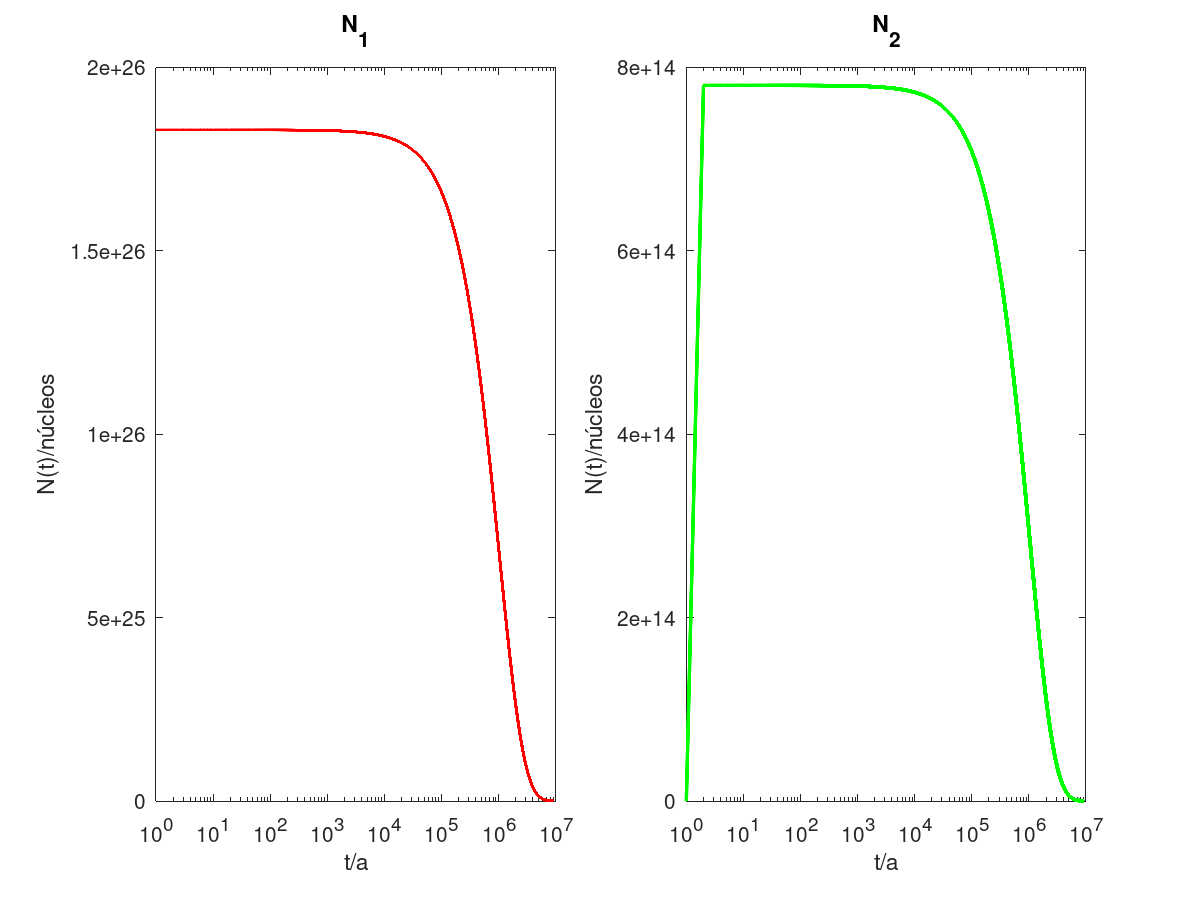
\includegraphics[scale=0.33]{/home/arias/Desktop/Research/u235_decay_chain_numsim/figuras/n1_n2.png}\label{n1n2}\caption{Curvas de desintegración de los núcleos $N_1$ y $N_2$ generadas por GNU Octave.}
\end{figure}

\begin{figure}[H]
	\centering
	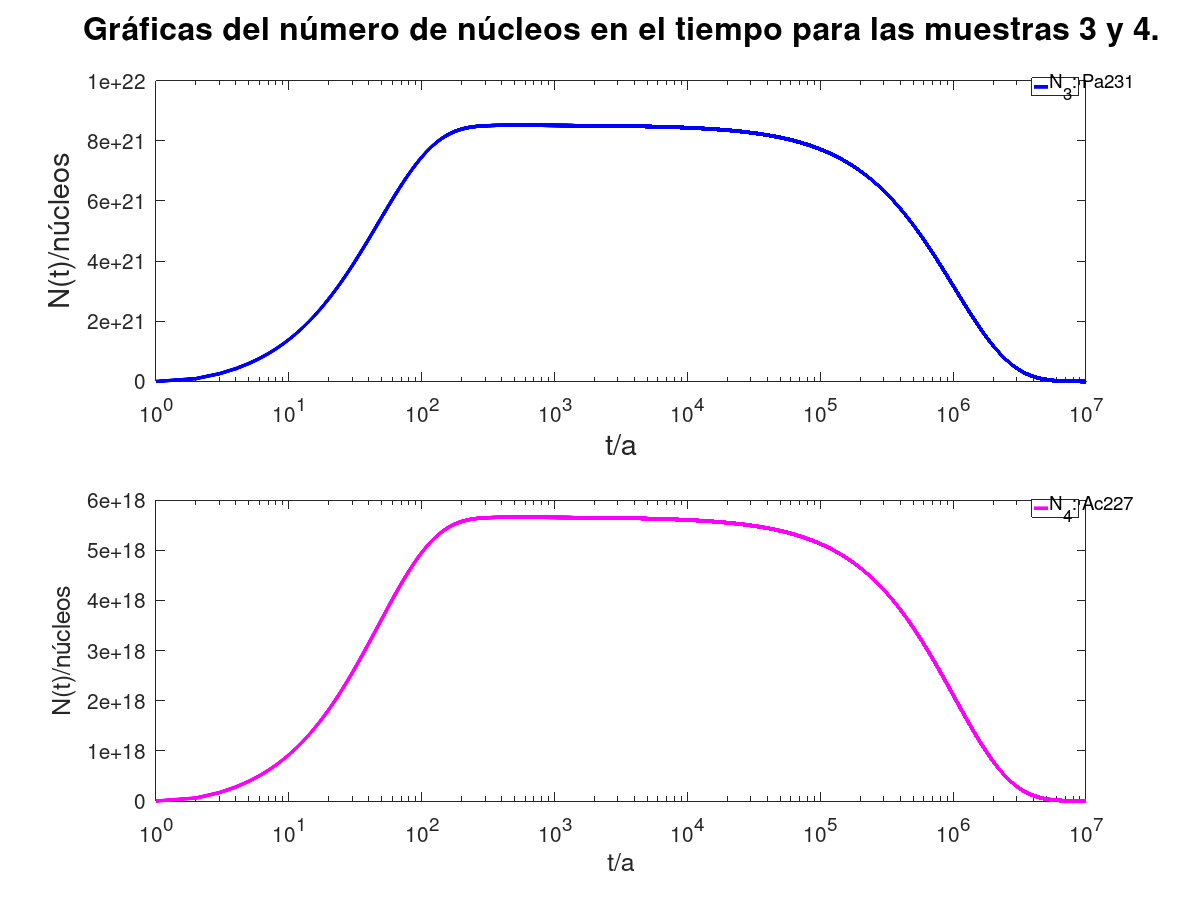
\includegraphics[scale=0.33]{/home/arias/Desktop/Research/u235_decay_chain_numsim/figuras/n3_n4.png}\label{n3n4}\caption{Curvas de desintegración de los núcleos $N_3$ y $N_4$ generadas por GNU Octave.}
\end{figure}

\begin{figure}[H]
	\centering
	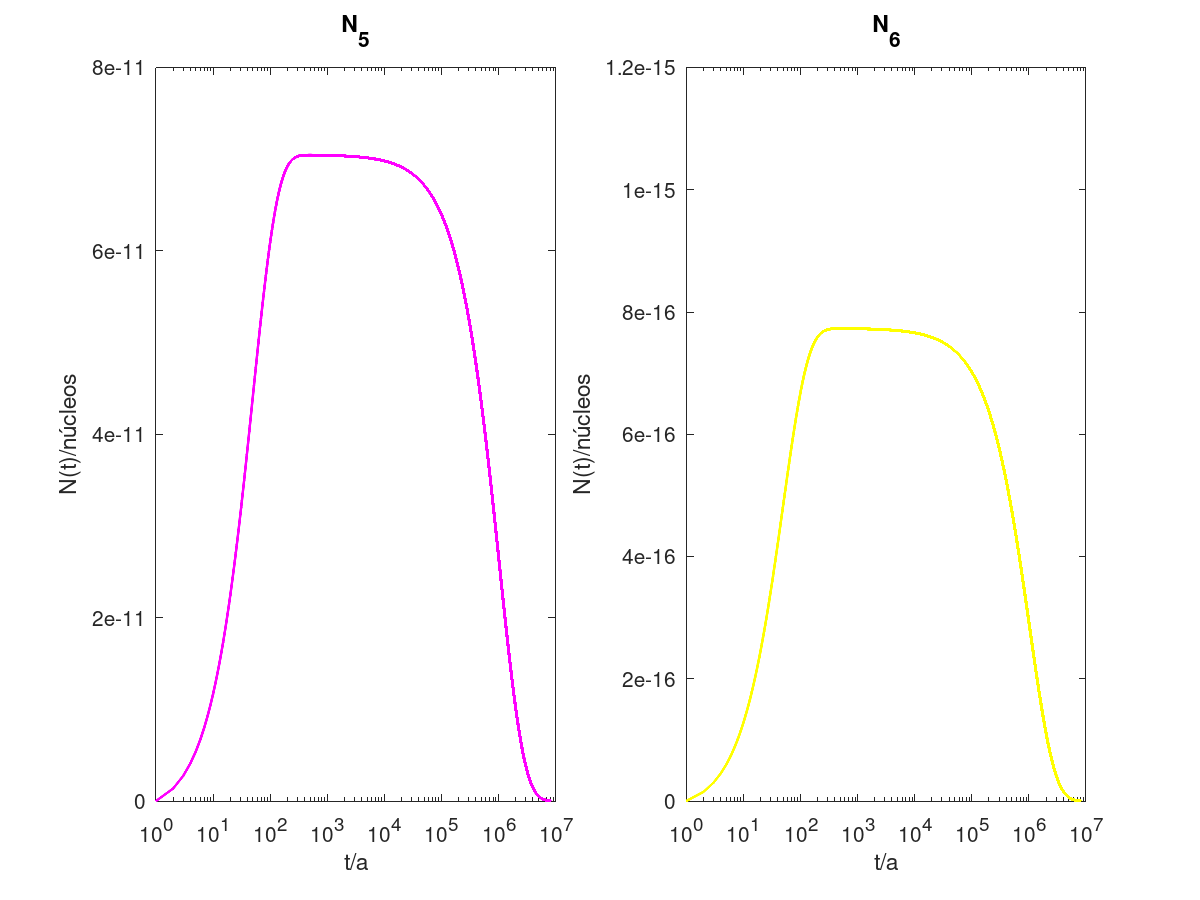
\includegraphics[scale=0.33]{/home/arias/Desktop/Research/u235_decay_chain_numsim/figuras/n5_n6.png}\label{n5n6}\caption{Curvas de desintegración de los núcleos $N_5$ y $N_6$ generadas por GNU Octave.}
\end{figure}

\begin{figure}[H]
	\centering
	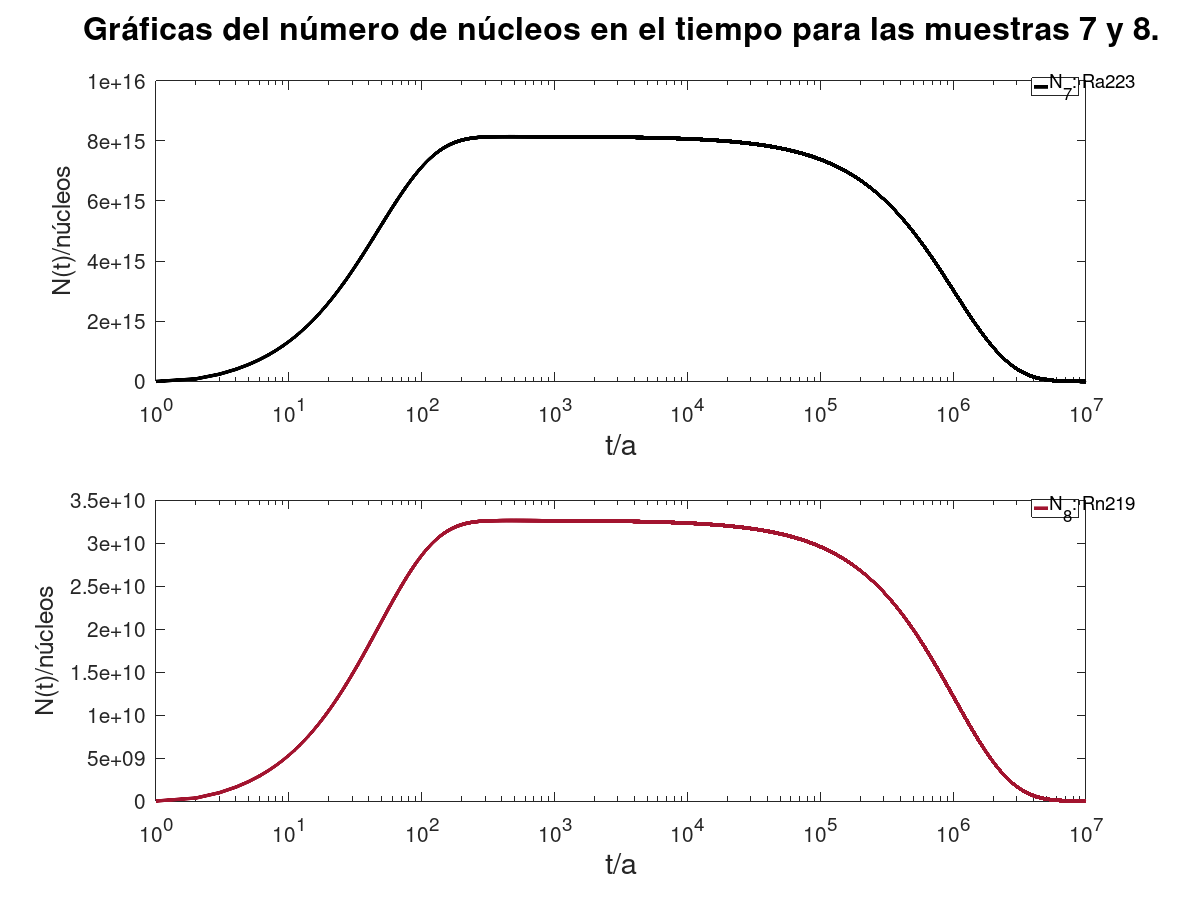
\includegraphics[scale=0.33]{/home/arias/Desktop/Research/u235_decay_chain_numsim/figuras/n7_n8.png}\label{n3n4}\caption{Curvas de desintegración de los núcleos $N_7$ y $N_8$ generadas por GNU Octave.}
\end{figure}

\begin{figure}[H]
	\centering
	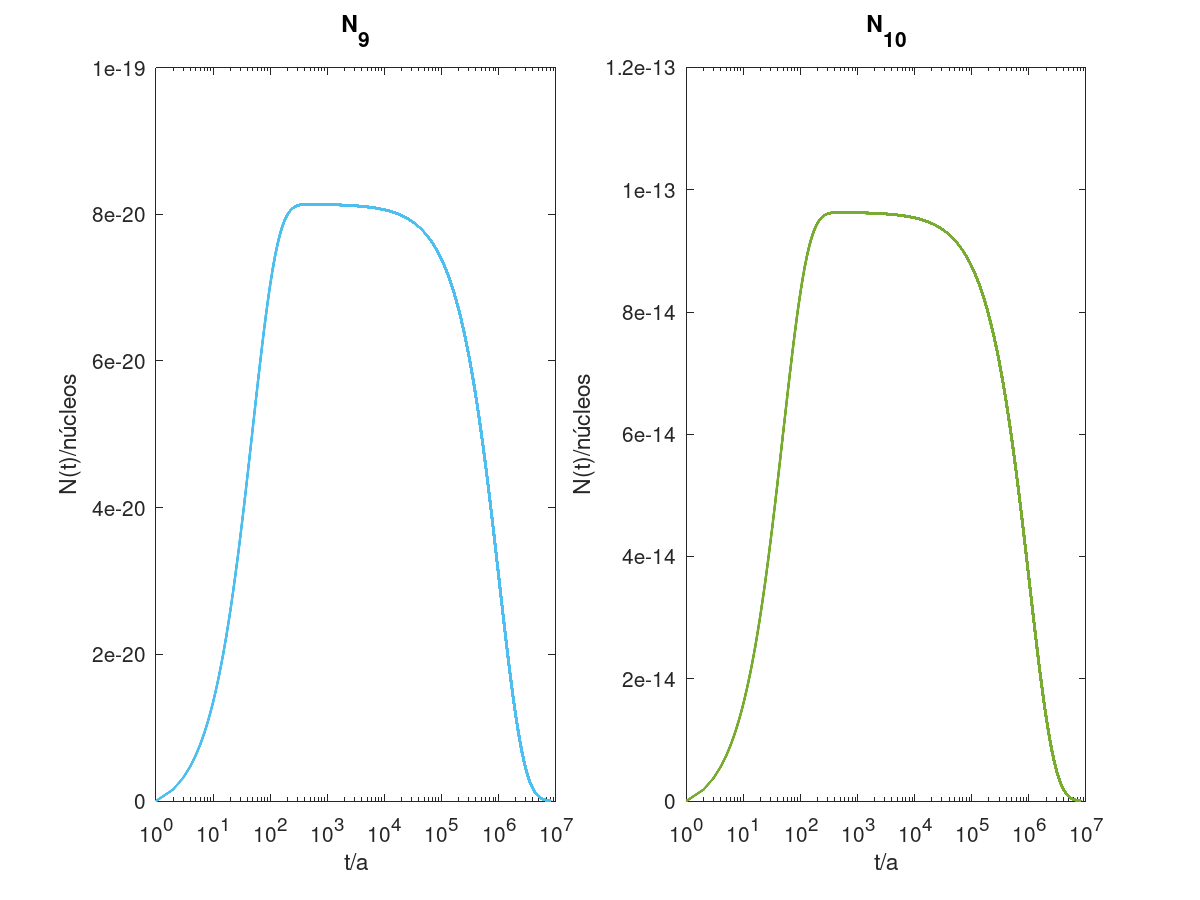
\includegraphics[scale=0.33]{/home/arias/Desktop/Research/u235_decay_chain_numsim/figuras/n9_n10.png}\label{n3n4}\caption{Curvas de desintegración de los núcleos $N_9$ y $N_{10}$ generadas por GNU Octave.}
\end{figure}

\begin{figure}[H]
	\centering
	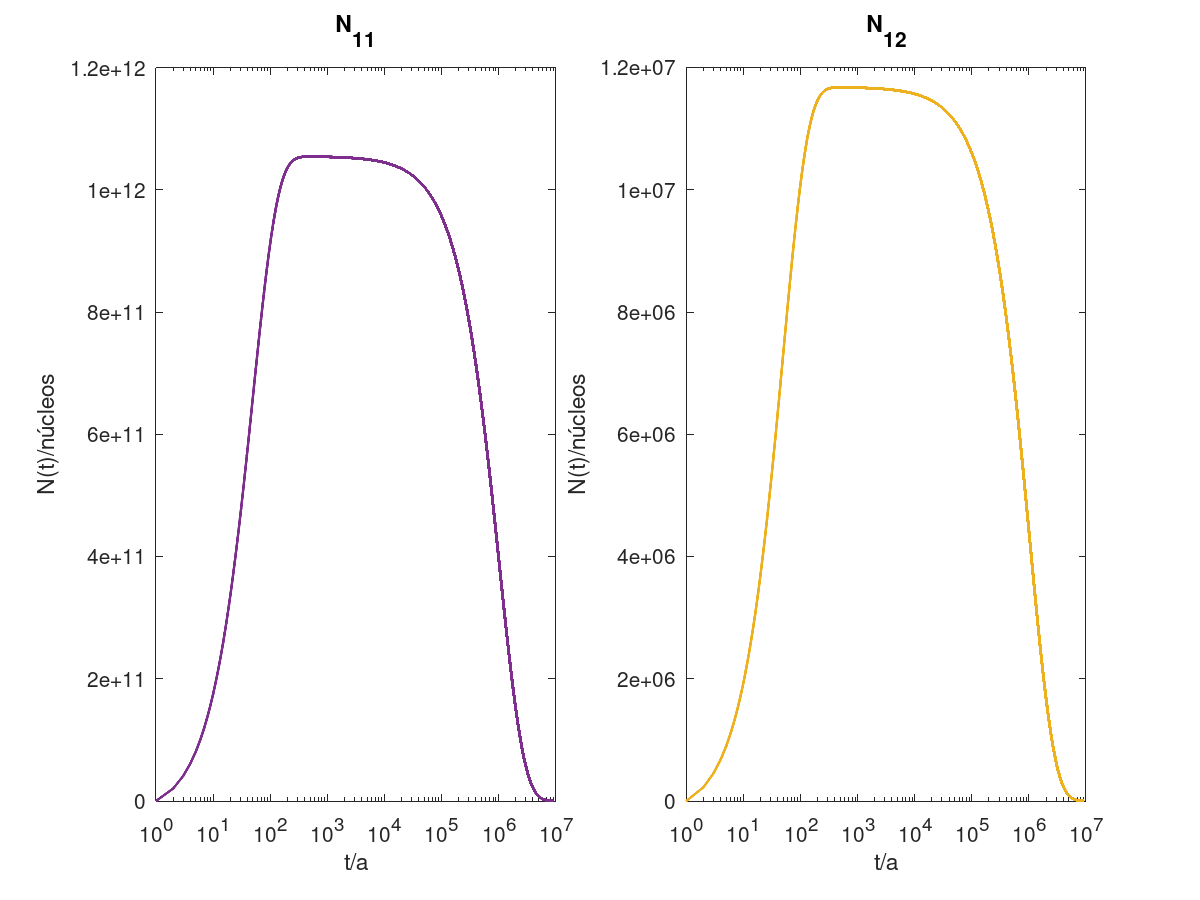
\includegraphics[scale=0.33]{/home/arias/Desktop/Research/u235_decay_chain_numsim/figuras/n11_n12.png}\label{n3n4}\caption{Curvas de desintegración de los núcleos $N_{11}$ y $N_{12}$ generadas por GNU Octave.}
\end{figure}

\begin{figure}[H]
	\centering
	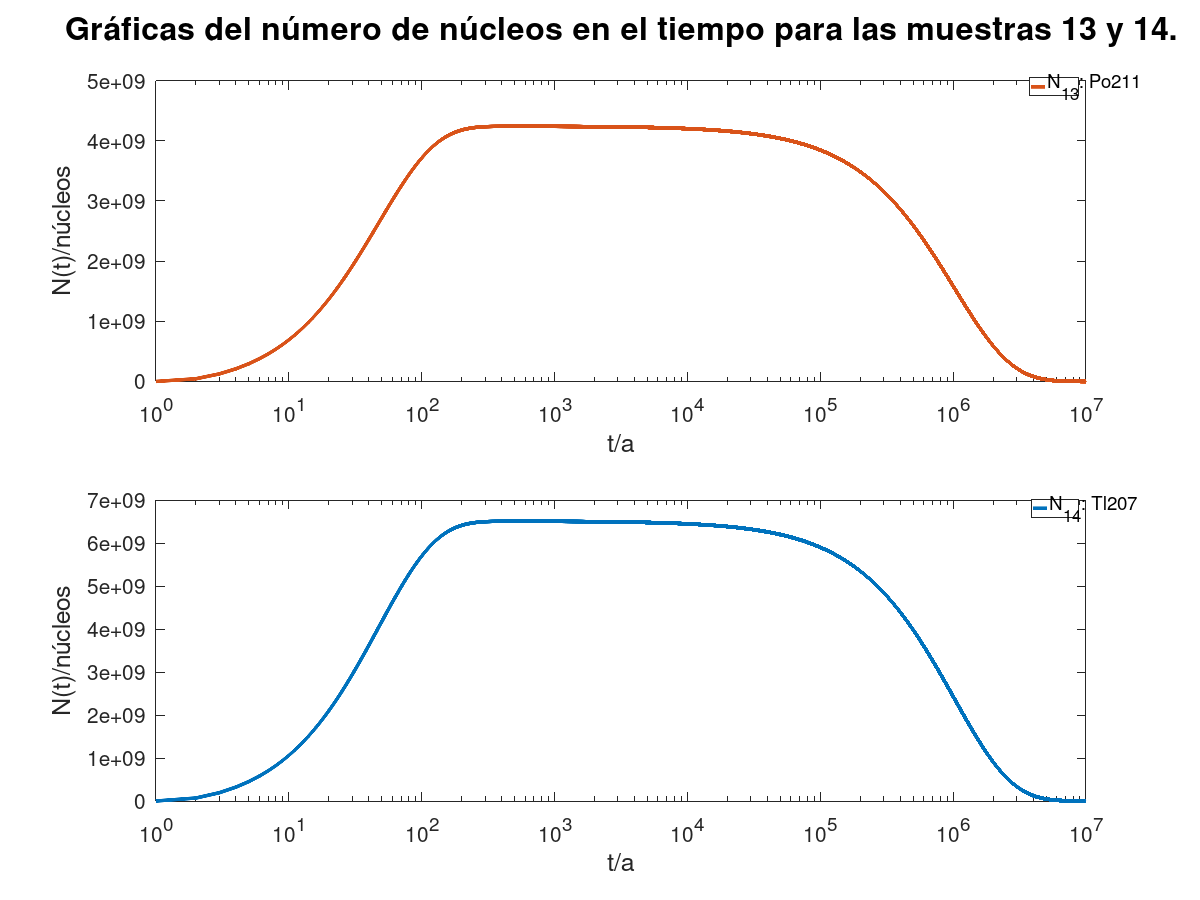
\includegraphics[scale=0.33]{/home/arias/Desktop/Research/u235_decay_chain_numsim/figuras/n13_n14.png}\label{n3n4}\caption{Curvas de desintegración de los núcleos $N_{13}$ y $N_{14}$ generadas por GNU Octave.}
\end{figure}

\begin{figure}[H]
	\centering
	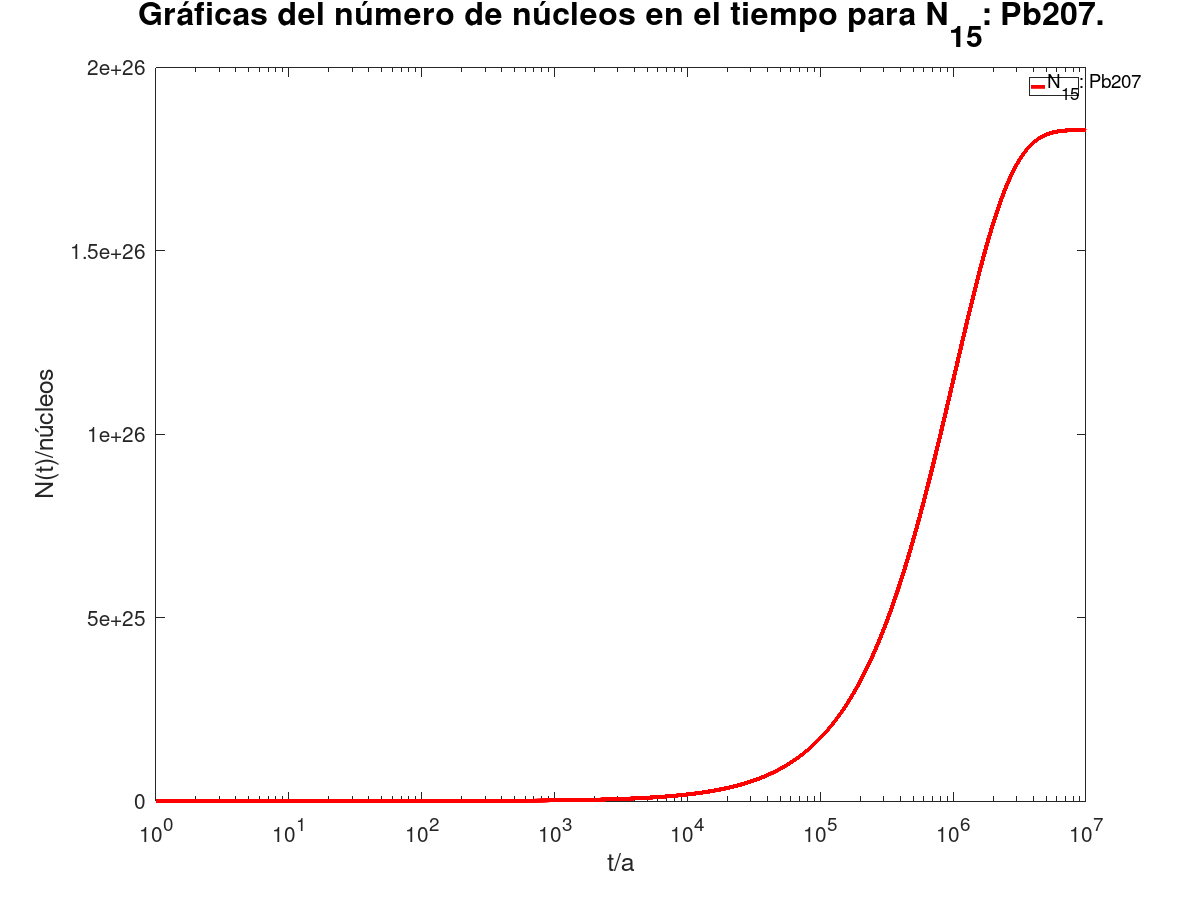
\includegraphics[scale=0.33]{/home/arias/Desktop/Research/u235_decay_chain_numsim/figuras/n15.png}\label{n15}\caption{Curva de desintegración del núcleo $N_{15}$ generada por GNU Octave.}
\end{figure}